\documentclass[
% -- opções da classe memoir --
12pt,				% tamanho da fonte
openright,			% capítulos começam em pág ímpar (insere página vazia caso preciso)
twoside,			% para impressão em frente e verso. Oposto a oneside
a4paper,			% tamanho do papel. 
% -- opções da classe abntex2 --
%chapter=TITLE,		% títulos de capítulos convertidos em letras maiúsculas
%section=TITLE,		% títulos de seções convertidos em letras maiúsculas
%subsection=TITLE,	% títulos de subseções convertidos em letras maiúsculas
sumario=tradicional, % configura estilo do sumário (comente estilo ABNTEX)
%subsubsection=TITLE,% títulos de subsubseções convertidos em letras maiúsculas
% -- opções da classe hyperref
hidelinks,          % oculta caixas e links coloridos
% -- opção de numerar continuamente as equações
%continuouseq,      % descomente para numeração contínua
% -- opção para citações e referências padrão IEEE	
%IEEE,				% citações e referências IEEE
% -- opções para citação utilizando classe abnt2cite
%alf,				% citação alfanumérica
num,				% citação numérica 
%overcite,			% citação no modo sobrescrito (se usar notas de rodapé, evite)
bibjustif,			% alinhamento justificado para as referências
brackets,			% citações com delimitador []
% -- opções do pacote babel --
english,			% idioma adicional para hifenização
brazil				% o último idioma é o principal do documento
]{article}       % utfprcopel.cls based on abnt2.cls


\usepackage{sbc-template}
\usepackage{float}
\usepackage{xcolor}
\usepackage{graphicx,url}
\usepackage{verbatim}                                       % Permite apresentar texto tal como escrito no documento, ainda que sejam comandos Latex
\usepackage{amsfonts, amssymb, amsmath}                     % Fontes e símbolos matemáticos
\usepackage{ae, aecompl}                                    % Fontes de alta qualidade
\usepackage{latexsym}                                       % Símbolos matemáticos
\usepackage[algoruled, portuguese]{algorithm2e}             % Permite escrever algoritmos em português
\usepackage[brazil]{babel}
\usepackage[utf8]{inputenc} 
\usepackage{indentfirst}
\usepackage{listings}
\usepackage{color}

\definecolor{dkgreen}{rgb}{0,0.6,0}
\definecolor{gray}{rgb}{0.5,0.5,0.5}
\definecolor{mauve}{rgb}{0.58,0,0.82}

\lstset{frame=tb,
  language=C,
  aboveskip=3mm,
  belowskip=3mm,
  showstringspaces=false,
  columns=flexible,
  basicstyle={\small\ttfamily},
  numbers=none,
  numberstyle=\tiny\color{gray},
  keywordstyle=\color{blue},
  commentstyle=\color{dkgreen},
  stringstyle=\color{mauve},
  breaklines=true,
  breakatwhitespace=true,
  tabsize=3
}
\renewcommand{\lstlistingname}{Código}% Listing -> Algorithm
\sloppy

\title{Reconhecimento do Gênero de Pessoas a Partir dos Sinais de suas Vozes}

\author{Kallil M. Caparroz\inst{1}, Rodrigo C. Anater\inst{2} }


\address{Universidade Tecnológica Federal do Paraná - Câmpus Pato Branco
  \email{kallil@alunos.utfpr.edu.br,
  rodrigoanater@alunos.utfpr.edu.br}
}

\begin{document} 

  \selectlanguage{brazil}
  \maketitle

\begin{abstract} 	
 	During the past two decades, the Machine Learning technique has become one of the main studies of information technology. With the increasing amount of information to be analyzed, there is a good reason to develop more and more computational algorythms to analyze these data. The objective of this work is to use different algorithms in the same dataset and compare which one is the best to be used.
\end{abstract}
     
\begin{resumo} 
 	Durante as duas últimas décadas, a técnica de Aprendizado de Máquinas tornou-se um dos principais estudos da tecnologia de informação. Com o aumento da quantidade de informações a serem analisadas, há uma boa razão para desenvolver mais e mais algoritmos computacionais a fim de analisar esses dados. O objetivo deste trabalho é usar diferentes algoritmos no mesmo conjunto de dados e comparar qual deles é o melhor a ser usado.   
\end{resumo}


\section{Introdução}
O termo \emph{Machine Learning} se refere à detecção, por parte do computador, em reconhecer padrões em uma base de dados.
Nas últimas décadas, tornou-se uma ferramenta fundamental para qualquer tarefa que requer a extração de informações de grandes conjuntos de dados. 

Estamos cercados por tecnologia baseada em \emph{Machine Learning}: Mecanismos de pesquisa aprendem como nos disponibilizar os melhores resultados, softwares anti-spam aprendem como filtrar nossos e-mails, assim como transações de cartões de créditos são mantidas em segurança por um software que aprende a detectar fraudes. \cite{shalev2014understanding}
Para tal, vários algoritmos conseguem fazer com que um computador possa automaticamente detectar os padrões de uma base de dados. 

Nesse trabalho será utilizada uma base de dados criada para identificar uma voz como masculina ou feminina baseada nas propriedades acústicas da voz e da fala. A base de dados consiste em 3 168 amostras de voz gravadas, coletadas de falantes masculinos e femininos, tendo 22 características, todas envolvendo a frequência sonora da fala, sendo algumas delas:

\begin{itemize}
	\item Frequência média (kHz)
	\item Desvio padrão da frequência
	\item Mediana da frequência (kHz)
	\item Centróide da frequência 
\end{itemize}

Para o reconhecimento dos padrões dessa base de dados serão utilizados duas técnicas: Regressão Linear e Máquinas de Vetores de Suporte.




\section{Regressão Linear}
O principal objetivo por trás da regressão linear é de estimar um valor $y \in \Re$ dado uma característica $x$.
Por exemplo, pode se estimar o valor de um estoque no dia seguinte de acordo com as vendas dos dias anteriores, os batimentos cardíacos de um atleta de acordo com a distância que percorreu, entre outras aplicações \cite{smola2008introduction}. 
 
 A Figura 1 mostra um bom exemplo de um método de regressão linear. Os pontos na figura são amostras obtidas das características $x$ da base de dados, o objetivo é criar uma função $f(x)$ que se aproxime da melhor forma dos valores observados.
\begin{figure}[H]
	\label{reg}
	\begin{centering}
		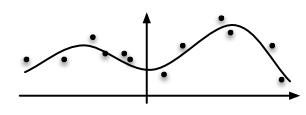
\includegraphics[width = 300pt]{img/regressao.png}
		\caption{Exemplo de regressão linear}
	\end{centering}	
	
\end{figure}

A função $f(x)$ utilizada pode ser representada pela forma:

$$ f(x) = b_0 + b_1*x_1 + b_1*x_1 + b_2*x_2 + ... + b_n*x_n $$

onde $x_{1,2,..n}$ correspondem às características da base de dados utilizada, $b_0$ corresponde à constante e $b_{1,2,..n}$ são os coeficientes. Os dois últimos são termos que o o método de regressão linear irá ajustar de forma a obter uma função que se aproxime dos valores dados pelo conjunto de treinamento.

Abaixo o código em linguagem python do processo de aprendizado da base de dados:
\begin{lstlisting}[language = python, numbers = left, ,backgroundcolor = \color{yellow!20}]
# Importing the libraries
import numpy as np
import pandas as pd

# Lista de Parametros
RATIO_TESTE_TREINO = 1000/3168
rs = np.random.randint(0,100)


#Importando a base de dados
dataset = pd.read_csv('voice.csv')
X = dataset.iloc[:, :-1].values
y = dataset.iloc[:, 20].values

#  Transformando as labels em numeros
from sklearn.preprocessing import LabelEncoder, OneHotEncoder
labelencoder_y = LabelEncoder()
y = labelencoder_y.fit_transform(y)
onehotencoder = OneHotEncoder(categorical_features = [0])
y = onehotencoder.fit_transform(y).toarray()
y = np.transpose(y)

# Dividindo a base de dados em treinamento e teste
from sklearn.cross_validation import train_test_split
X_train, X_test, y_train, y_test = train_test_split(X,y,test_size=RATIO_TESTE_TREINO, stratify=y)

# Metodo de regressao linear simples
from sklearn.linear_model import LinearRegression
regressor = LinearRegression()
regressor.fit(X_train, y_train)

#Prevendo os resultados da base de testes
y_pred = regressor.predict(X_test)
y_pred = np.round(y_pred)

#Calcular a precisao dos resultados
from sklearn.metrics import accuracy_score
print('Accuracy simple linear regression: %.2f\n' % accuracy_score(y_test, y_pred))
\end{lstlisting}  

Com uma base de treinamento de 2000 instâncias e uma base de treino de 1 168 instâncias, a precisão desse método foi entre 96\% e 97\%.
\section{SVM}

Máquinas de vetores suporte, ou SVM (do inglês, \emph{Support Vector Machines}) é um método de aprendizado de máquina supervisionado, binário e não probabilístico, que se baseia na criação de um hiperplano ótimo para a divisão entre classes. A criação do plano se baseia não em todos os elementos, mas sim em um grupo especifico, os chamados "vetores suporte", de onde vem o nome do método. Esse vetores suporte são os de mais difícil classificação, uma vez que se encontram mais próximos dos elementos do outro grupo.

O SVM, quando linear, funciona de maneira semelhante a outros métodos que se utilizam da criação de uma superfície de decisão, porem, tem a capacidade de se adaptar para a classificação de dados não linearmente separáveis através do truque de kernel, que permite o aumento da dimensionalidade dos dados, de forma à possibilitar a separação dos mesmos.

Por sua natureza, o método SVM mantem uma boa funcionalidade em espaços com grande número de dimensões, inclusive quando esse número é superior ao número de elementos. Dispões também de versatilidade, se adaptando à diferentes distribuições através da escolha do kernel. A principal desvantagem está na grande complexidade do método, tanto computacional, podendo exigir uma grande quantidade de processamento para a criação do hiperplano de separação, quanto teórica, apresentando um grande desafio na abstração matemática de seu funcionamento, uma vez que pode funcionar em um alto números de dimensões.

Para a utilização prática do SVM, o primeiro parâmetro a ser analisado é o \textbf{C}, referente às chamadas \emph{slack variables}, que permitem que a superfície de decisão treinada aceite erros no treino em troca de uma maior simplicidade na superfície de decisão. O valor base de \textbf{C} é 1, valores menores criam uma superfície mais simples, enquanto valores maiores buscam uma classificação mais exata, aceitando um maior numero de vetores suporte, porem com o risco de causar um \emph{overfitting} do modelo.

Em seguida, deve-se escolher o kernel. Em um conjunto de dados linearmente separável, pode ser utilizado o SVM linear, ou seja, sem a utilização de um kernel. Porém, em muitos casos, os dados não são tão bem comportados, e é necessária a aplicação do truque de kernel. O truque se baseia na aplicação de uma operação vetorial sobre os elementos, de forma que o conjunto ocupe um maior número de dimensões, onde este possa ser separado. Para distribuições discretas, é possível até mesmo a adição de uma dimensão para cada elemento, de forma a garantir a separabilidade do conjunto. Já em dados que seguem uma distribuição continua, como é o caso, é realizado um produto interno
.
As escolhas mais comuns de kernel são a função de base radial (RBF), polinomial e sigmoide. O kernel RBF aplica uma transformação na forma de uma curva normal sobre os dados, que normalmente permite uma melhor separação de dados provenientes de medições reais, como é o caso. O kernel polinomial aplica um polinômio de ordem N, que define o formato da curva. O kernel sigmoidal aplica uma sigmoide, sendo recomendada para alguns casos específicos onde os dados seguem uma certa distribuição probabilística. Em geral, é sugerido o teste de diferentes kerneis, começando pelo RBF, devido à sua menor complexidade computacional.

Uma vez escolhido um kernel, surge um terceiro parâmetro de grande importância, o \textbf{gamma}, referente ao coeficiente da função do kernel. Uma forma de se avaliar a ação do \textbf{gamma} é como um parâmetro que define a área de influencia de cada vetores suporte, de forma inversa ao seu valor. Valores altos de \textbf{gamma} reduzem a influencia dos vetores suporte, causando um \emph{overfitting} do modelo, enquanto valores pequenos podem causar uma restrição excessiva do modelo, de forma que não consiga acompanhar o comportamento dos dados. O valor padrão de \textbf{gamma} pelo scikit learn é o inverso do numero de característica, de forma à balancear a influencia.

Para o problema analisado, os melhores resultados foram obtidos com a utilização do kernel RBF, como é de se esperar, uma vez que os dados devem seguir uma distribuição normal, pois foram extraídos de uma situação real. Para o valor de C, o resultado apenas sofreu com escolhas muito baixas ou extremas, sendo que o valor padrão de um resultou no melhor resultado. Finalmente, para o gamma, o valor de 0.05, referente às 20 características também resultou no melhor caso analisado. Com esses parâmetros, foi obtida uma precisão de 98\% de acertos.


\begin{lstlisting}[language = python, numbers = left, ,backgroundcolor = \color{yellow!20}]

# Importing the libraries
import numpy as np
import pandas as pd

# Lista de Parametros
RATIO_TESTE_TREINO = 0.3
rs = 13#np.random.randint(0,100)


#Importando a base de dados
dataset = pd.read_csv('voice.csv')
X = dataset.iloc[:, :-1].values
y = dataset.iloc[:, 20].values

#  Transformando as labels em numeros
from sklearn.preprocessing import LabelEncoder, OneHotEncoder
labelencoder_y = LabelEncoder()
y = labelencoder_y.fit_transform(y)
onehotencoder = OneHotEncoder(categorical_features = [0])
y = onehotencoder.fit_transform(y).toarray()
y = np.transpose(y)

# Dividindo a base de dados em treinamento e tes
from sklearn.cross_validation import train_test_split
X_train, X_test, y_train, y_test = train_test_split(X,y,test_size=RATIO_TESTE_TREINO, stratify=y)

# Normalizacao:
from sklearn.preprocessing import StandardScaler
sc = StandardScaler()
sc.fit(X_train)
X_train_std = sc.transform(X_train)
X_test_std = sc.transform(X_test)


#%% SVM
from sklearn import svm

mvs = svm.SVC(C=1, kernel='rbf', gamma=0.05)

mvs.fit(X_train_std, y_train)
y_pred = mvs.predict(X_test_std)

from sklearn.metrics import accuracy_score
print('Accuracy SVM: %.2f\n' % accuracy_score(y_test, y_pred))



\end{lstlisting}
\input{tex/conclusao.tex}



\bibliographystyle{sbc}
\bibliography{sbc-template}
\end{document}